\chapter{Experiments}
\label{chapter:experiments}

In this chapter we discuss the implementation details of the project, the training process for the agents and the results we have obtained.

\section{Implementation}

As was mentioned in chapter \ref{chapter:introduction}, this project is a continuation of previous works by other students. As such, we have decided to use the existing codebase as a starting point. The entire code, as well as the custom mini-games and trained models, is available in our public GitHub repository\footnote{\url{https://github.com/DavidPerezGomez/tfm-rl-starcraft2}}.

\subsection{Agent structure}
\label{sec:agent_structure}

Our agents implement the Deep Q-Learning algorithm described in section \ref{sec:dql}. They include two neural networks (main and target) to learn to estimate the value of state-action pairs, and a replay buffer to store previous experiences as training samples for the networks. They also implement the $\epsilon$-greedy method to favour exploration during the entire training process.

\subsubsection*{Networks}

The neural networks, including optimizer and scheduler, are implemented using PyTorch. They are fully connected multilayer perceptrons. Since the size and shape of neural networks can have a large impact on their performance and ability to learn, we have defined three increasingly complex configurations for the hidden layers to use throughout the project:

\begin{itemize}
    \item \textbf{Medium:} Has four hidden layers with 128, 128, 64 and 32 neurons respectively.
    \item \textbf{Large:} Has five hidden layers with 256, 128, 128, 64 and 32 neurons respectively.
    \item \textbf{Extra large:} Has size hidden layers with 512, 256, 128, 128, 64 and 32 neurons respectively.
\end{itemize}

\subsubsection*{Action implementation}

To implement the actions described in section \ref{sec:action_space} we use the following raw actions from the PySC2 API:

\begin{itemize}
    \item \textbf{\texttt{Harvest\_Gather\_unit}:} Given a worker unit and a mineral patch, it commands the worker to harvest minerals from the path.
    \item \textbf{\texttt{Train\_SCV\_quick}:} Given a Command Center, it begins training an SCV in the Command Center.
    \item \textbf{\texttt{Build\_CommandCenter\_pt}:} Given an SCV and a coordinates point in the map, it commands the SCV to build a Command Center on the specified position.
    \item \textbf{\texttt{Build\_SupplyDepot\_pt}:} Given an SCV and a coordinates point in the map, it commands the SCV to build a Supply Depot on the specified position.
    \item \textbf{\texttt{Build\_Barracks\_pt}:} Given an SCV and a coordinates point in the map, it commands the SCV to build a Barracks on the specified position.
    \item \textbf{\texttt{Train\_Marine\_quick}:} Given a Barracks, it begins training a Marine in the Barracks.
    \item \textbf{\texttt{Attack\_unit}:} Given two units, it commands the first one to move and attack towards the second one.
\end{itemize}

\subsubsection*{Action masking}

\begin{figure}[t]
    \begin{equation*}
        \begin{bmatrix}
        q_1 \\ q_2 \\ q_3 \\ q_4 \\ \vdots \\ q_n
        \end{bmatrix}
        \times 
        \begin{bmatrix}
        1 \\ 0 \\ 0 \\ 1 \\ \vdots \\ 0
        \end{bmatrix}
        \Rightarrow 
        \begin{bmatrix}
        q_1 \\ -\infty \\ -\infty \\ q_4 \\ \vdots \\ -\infty
        \end{bmatrix}
    \end{equation*}
\caption{Application of action masking}
\label{fig:action_masking}
\end{figure}

Action masking is a technique used to prevent a reinforcement learning agent from selecting actions that would be invalid for the current state, such as training a Marine without enough resources or an available Barracks, for example. It has been shown to improve learning efficiency in complex action spaces \cite{Huang:2022}. The previous work implemented action masking during exploitation, but not during training. Instead, if an invalid action was selected, it would be transformed into a \texttt{NO\_OP} action, but the agent would still learn based on the action it originally selected.

For this project, we have decided to apply action masking during training as well. Part of the reason for this is that using action masking only during inference means that the agent will sometimes be prevented from following the policy that it has learned, which prevent us from accurately evaluating said policy. Another reason is that the conversion from invalid actions to \texttt{NO\_OP} during training can cause the agent to learn to use invalid actions as a proxy for the \texttt{NO\_OP} action. This would not be a desired behavior, since we want the agent to be deliberate when selecting actions.

To implement action masking, whenever an agent needs to select an action we use custom logic to determine which actions would be invalid for the current state and apply that mask to the q-values generated by the neural network, converting the values associated with the invalid actions into negative infinity (figure \ref{fig:action_masking}). The agent then selects the action with the highest q-value, which necessarily excludes the invalid actions. Since the \texttt{NO\_OP} is always valid, the agents will always have at least one valid action available.

It should be noted that whenever we make use of random agents (be it as baselines to compare the performance of RL agents or as opponents in versus maps), we also apply action masking, allowing them to select randomly only from the set of valid actions.

\subsubsection*{Action frequency}

In section \ref{sec:pysc2} we explained how PySC2 allows us to configure how often the agent will be able to act on the environment. Setting the action frequency too low can obviously lead to poor performance, since the agent would be too slow to react to events taking place in the game. Setting it too high, however, can present its own set of challenges. For one, it amplifies the sparse and long-term reward issues present in the environment: the more observations and actions the agent takes, the more \say{perceived} time it will take for long-term investments to pay off. Second, StarCraft II is a relatively slow paced game, where situations don't change drastically in an instant. Two observations taken in a very short time will be almost identical in most situations, slowing down the training process.

In the end, we have settled on acting every 32 game ticks (2 in-game seconds), which we think strikes a decent balance.

\subsubsection*{Custom scenarios}

Lastly, we found that the mini-games distributed with PySC2 didn't fit with the needs and limitations of our different agents. For that reason, we have used the StarCraft II map editor to create our own custom maps. These are described in section \ref{sec:training} alongside each of the agents that were trained in them.

\subsection{Hierarchical model}

Our Hierarchical model consists of four different agents: one high-level manager and three lower-level sub-agents. The main agent, also called game manager, is tasked with selecting which of the sub-agents will decide the next several actions. For that purpose, instead of the set of actions described in section \ref{sec:action_space}, it works with a different, exclusive list of actions:

\begin{itemize}
    \item \textbf{\texttt{EXPAND\_BASE}:} Delegate the action selection to the base manager sub-agent.
    \item \textbf{\texttt{EXPAND\_ARMY}:} Delegate the action selection to the recruit manager sub-agent.
    \item \textbf{\texttt{ATTACK}:} Delegate the action selection to the attack manager sub-agent.
\end{itemize}

Action masking is not applied to these action.

The main agent will also implement a temporal extension of five steps, meaning that it will act only every five steps (160 game ticks, 10 in-game seconds), as explained in \ref{sec:hrl}.

\subsubsection*{Attack manager sub-agent}

The attack manager sub-agent is in charge of using the Marine army to destroy the enemy units and structures. It has access to the following actions:

\begin{multicols}{2}
\begin{itemize}
    \item \textbf{\texttt{NO\_OP}}
    \item \textbf{\texttt{ATTACK\_CLOSEST\_BUILDING}}
    \item \textbf{\texttt{ATTACK\_CLOSEST\_WORKER}}
    \item \textbf{\texttt{ATTACK\_CLOSEST\_ARMY}}
    \item \textbf{\texttt{ATTACK\_BUILDINGS}}
    \item \textbf{\texttt{ATTACK\_WORKERS}}
    \item \textbf{\texttt{ATTACK\_ARMY}}
\end{itemize}
\end{multicols}

It can choose what type of enemy unit to attacks and whether to target whichever is closest or the biggest cluster of enemies. Although it has access to the \texttt{NO\_OP} action, it will be prevented from selecting it, through action masking, unless every other action is unavailable (in the case that the agent has no marines or there are no enemy units). This is because the game has an automatic targeting system where an idle combat unit that is in range of enemy units will start attacking them while prioritizing targets according to the game's AI. Using this, the agent could learn a \say{launch and forget} strategy by sending the marines to attack the enemy and then simply waiting and letting the game's AI control most of the fight. Since our goal is to keep the environment and action space more complex than the previous work, we want the agent to be forced to take a more active role.

\subsubsection*{Recruit manager sub-agent}

The recruit manager sub-agent is in charge of training the Marine army by creating Barracks and recruiting Marines. It has access to the following actions:

\begin{multicols}{2}
\begin{itemize}
    \item \textbf{\texttt{NO\_OP}}
    \item \textbf{\texttt{HARVEST\_MINERALS}}
    \item \textbf{\texttt{BUILD\_SUPPLY\_DEPOT}}
    \item \textbf{\texttt{BUILD\_BARRACKS}}
    \item \textbf{\texttt{RECRUIT\_MARINE}}
\end{itemize}
\end{multicols}

Since performing an action to build structures while there are no idle workers will cause a harvesting worker to stop gathering minerals, the agent has the ability to send workers back to harvesting, so as to not cripple the resource economy by accident, specially when working by itself during training.

\subsubsection*{Base manager sub-agent}

The base manager sub-agent is in charge of developing the resource economy by creating more workers and Command Centers. It has access to the following actions:

\begin{multicols}{2}
\begin{itemize}
    \item \textbf{\texttt{NO\_OP}}
    \item \textbf{\texttt{HARVEST\_MINERALS}}
    \item \textbf{\texttt{BUILD\_COMMAND\_CENTER}}
    \item \textbf{\texttt{RECRUIT\_SCV\_0}}
    \item \textbf{\texttt{RECRUIT\_SCV\_1}}
    \item \textbf{\texttt{RECRUIT\_SCV\_2}}
    \item \textbf{\texttt{BUILD\_SUPPLY\_DEPOT}}
\end{itemize}
\end{multicols}

It has the ability to build Supply Depots because the amount of workers is also limited by the supply resource. Although each Command Center provides some supply, it is not enough to reach the optimal worker amount, and some Supply Depots are necessary at some point.

\section{Training}
\label{sec:training}

Training the RL agents proved to be more challenging than expected. We have gone through many revision of the training mini-games and reward signals for each for the sub-agents, main hierarchical agent and single agent. In general, the agents had trouble converging, often finding a good solution part way through the training, only to then collapse and spiral toward considerably worse policies as the training continued. We had to make use of frequent checkpoints to get versions of the agents with effective policies. The increasing values for the training loss that can be seen in appendix \ref{app:stats} suggest that the frequency at which we synchronize the target network with the main network may be too high, but we were unable to explore further due to time limitations.

\begin{figure}[t]
    \centering
    \begin{subfigure}[b]{0.45\textwidth}
        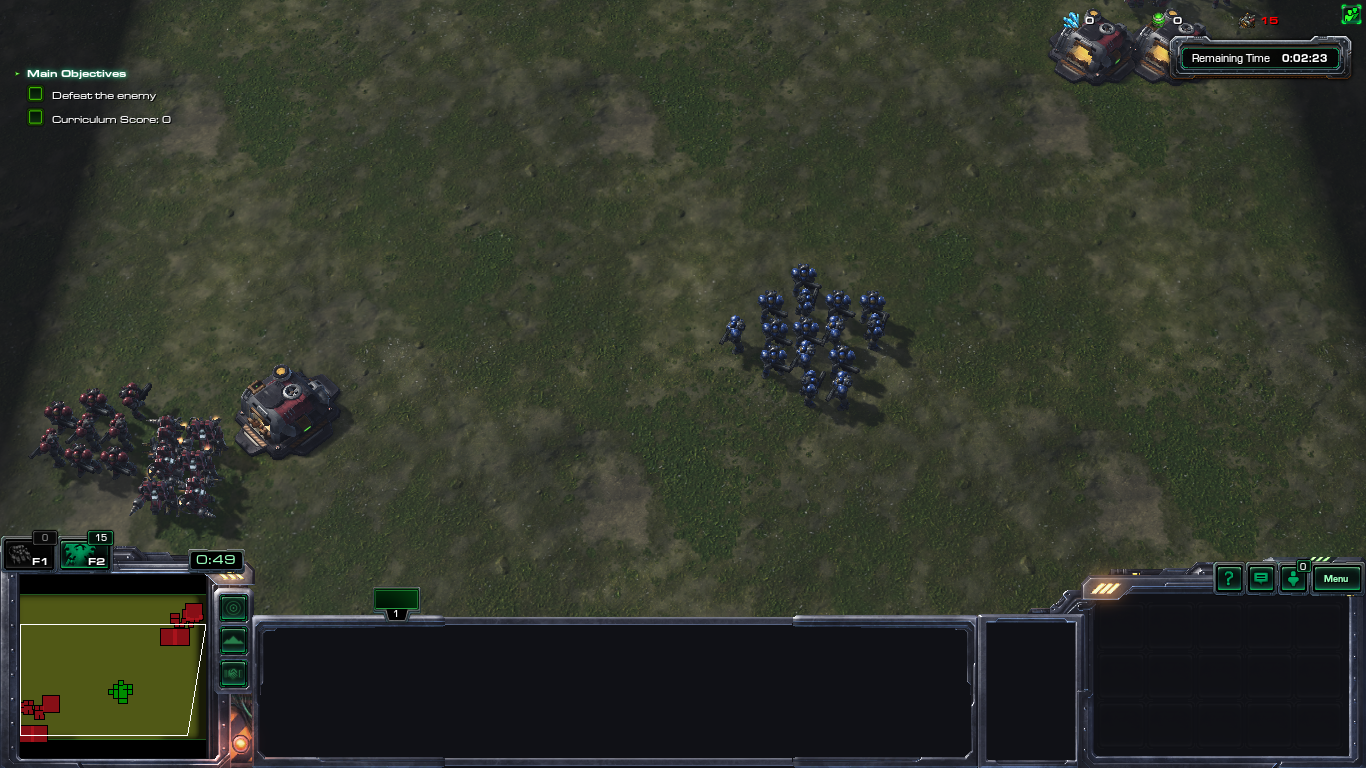
\includegraphics[width=1\textwidth]{figs/DefeatBases.png}
        \caption{\texttt{DefeatBases} mini-game}
        \label{fig:DefeatBases}
    \end{subfigure}
    \hfill
    \begin{subfigure}[b]{0.45\textwidth}
        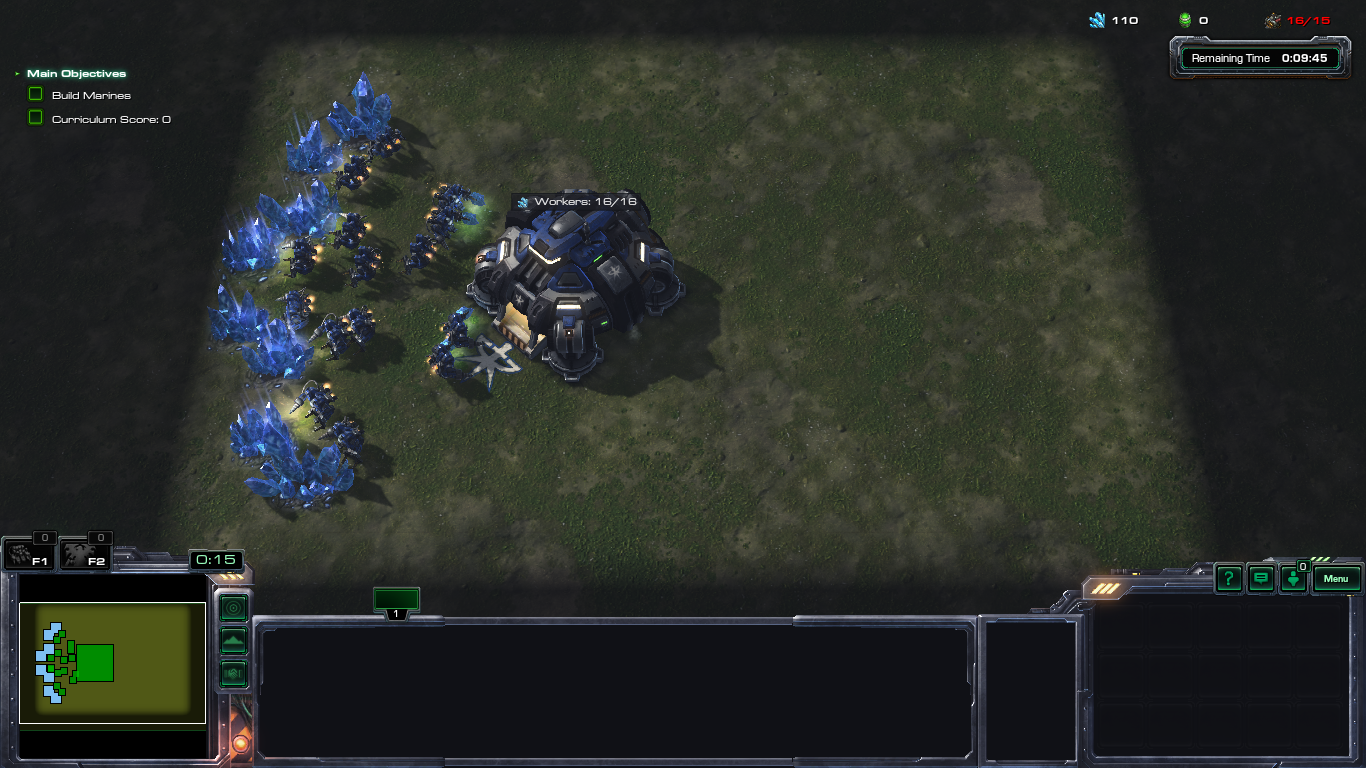
\includegraphics[width=1\textwidth]{figs/BuildMarinesFixed.png}
        \caption{\texttt{BuildMarinesFixed} mini-game}
        \label{fig:BuildMarinesFixed}
    \end{subfigure}
    \hfill
    \begin{subfigure}[b]{0.45\textwidth}
        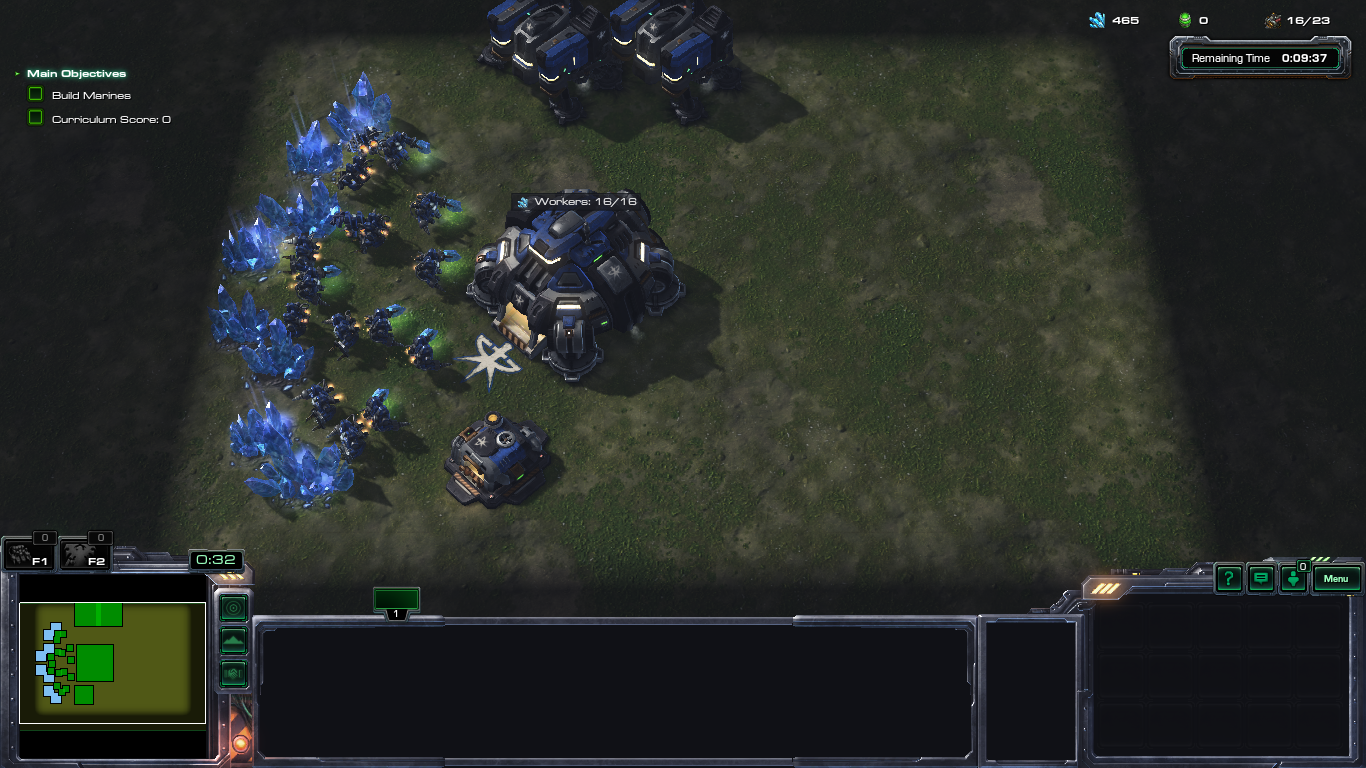
\includegraphics[width=1\textwidth]{figs/BuildMarinesRandom.png}
        \caption{\texttt{BuildMarinesRandom} mini-game}
        \label{fig:BuildMarinesRandom}
    \end{subfigure}
    \hfill
    \begin{subfigure}[b]{0.45\textwidth}
        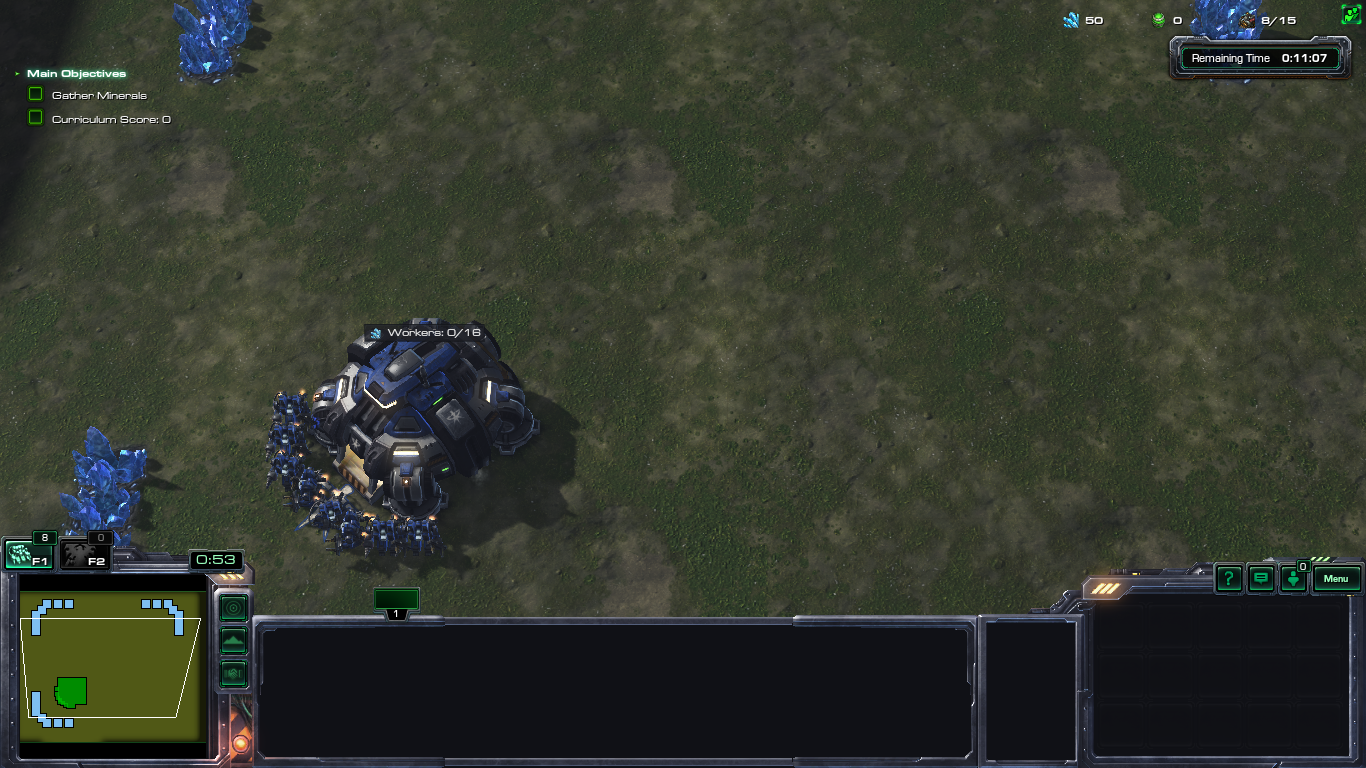
\includegraphics[width=1\textwidth]{figs/SaturateHarvesters.png}
        \caption{\texttt{SaturateHarvesters} mini-game}
        \label{fig:SaturateHarvesters}
    \end{subfigure}
    \caption{Custom mini-games}
\end{figure}

\subsection{Attack manager}

The pre-existing PySC2 mini-games that center around combat focus only on enemy combat units, and none include workers or structures, which we want so that the agent gets more complete observations and learns the new attack actions with specific targets. Additionally, the enemy units used are always from the Zerg race, which doesn't represent the type of opposition that the agent will find in the final versus map. For those reasons, we have created a new mini-game called \texttt{DefeatBases} (figure \ref{fig:DefeatBases}).

The objective of this mini-game is to destroy two small enemy bases. The agent starts with a group of Marines of variable size placed a random point close to the center of the map. The enemy bases consist of three Supply Depots, a small random number of SCVs and a small random number of Marines, randomly positioned on opposite corners of the map. The enemy Marines are programmed to attack any units that damage nearby buildings and the SCVs are programmed to repair nearby buildings. The number of ally and enemy Marines is set up so that the allies can destroy both bases reliably if played correctly. The map ends when all enemy buildings have been destroyed or after 3 minutes.

For this agent, we have created a reward signal that encourages destroying the enemy units and structures quickly while losing as few of the agent's own marines as possible. The score calculated for each step is the difference in health of all ally units and all enemy units. The reward for the agent is the change in score from the previous step, with an additional flat penalty to encourage faster episodes. The agent has to prioritize targeting enemy Marines, then SCVs and then buildings, and to focus on a single base at a time to maximize the reward.

$$
r(t) = \Delta(\texttt{health\_allies}_{t} - \texttt{health\_enemies}_{t}) - \texttt{step\_cost}
$$

The sub-agent uses a medium neural network and has been trained for 6147 steps (150 episodes). Figure \ref{fig:DefeatBases_scores} shows the scores obtained by the trained agent during exploitation compared to the ones obtained by a random agent.

\begin{figure}[t]
    \centering
    \begin{subfigure}[b]{0.48\textwidth}
        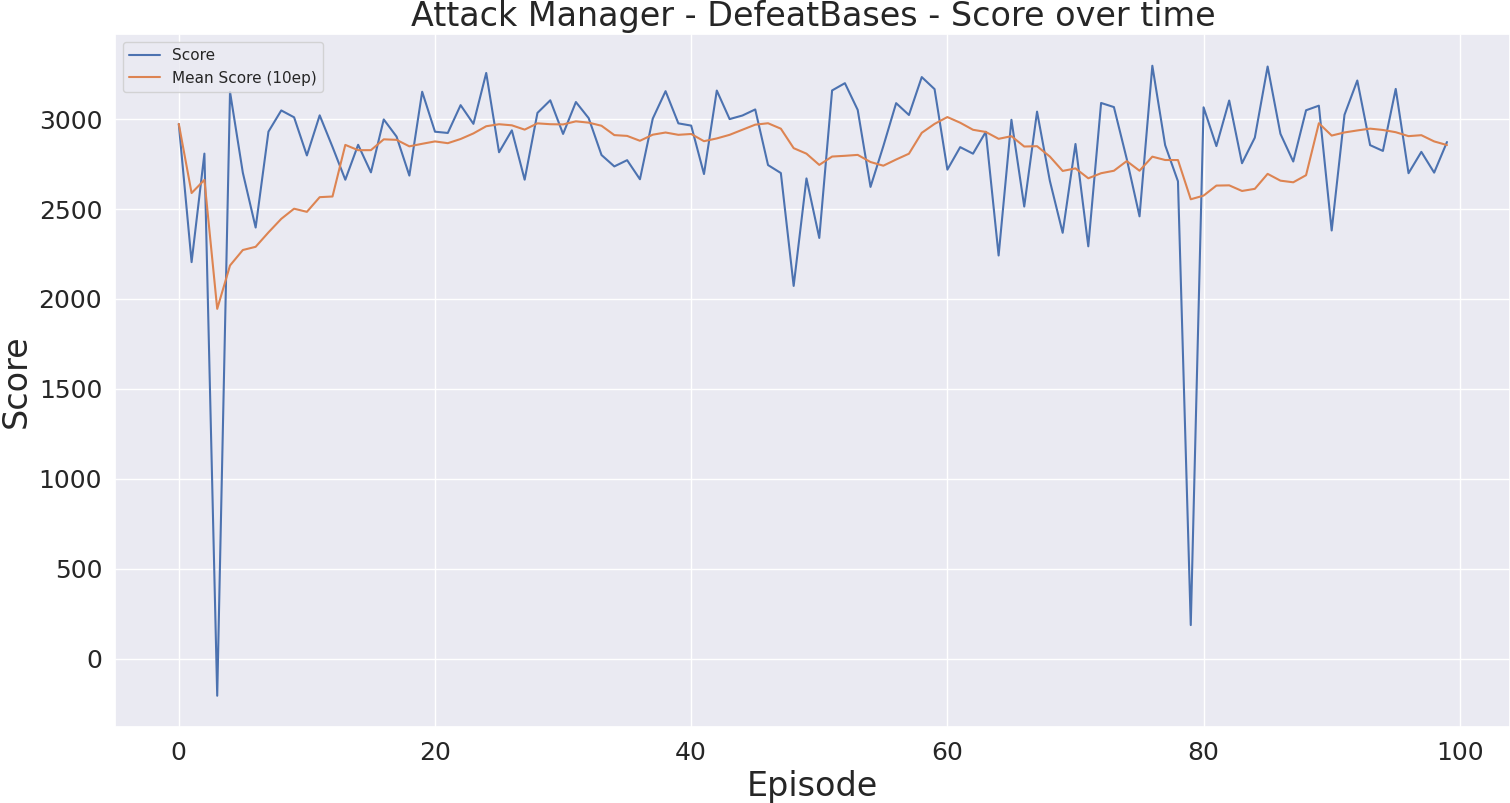
\includegraphics[width=1\textwidth]{figs/multi_dqn_army_attack_manager/exploit/score.png}
        \caption{Attack manager sub-agent score}
    \end{subfigure}
    \hfill
    \begin{subfigure}[b]{0.48\textwidth}
        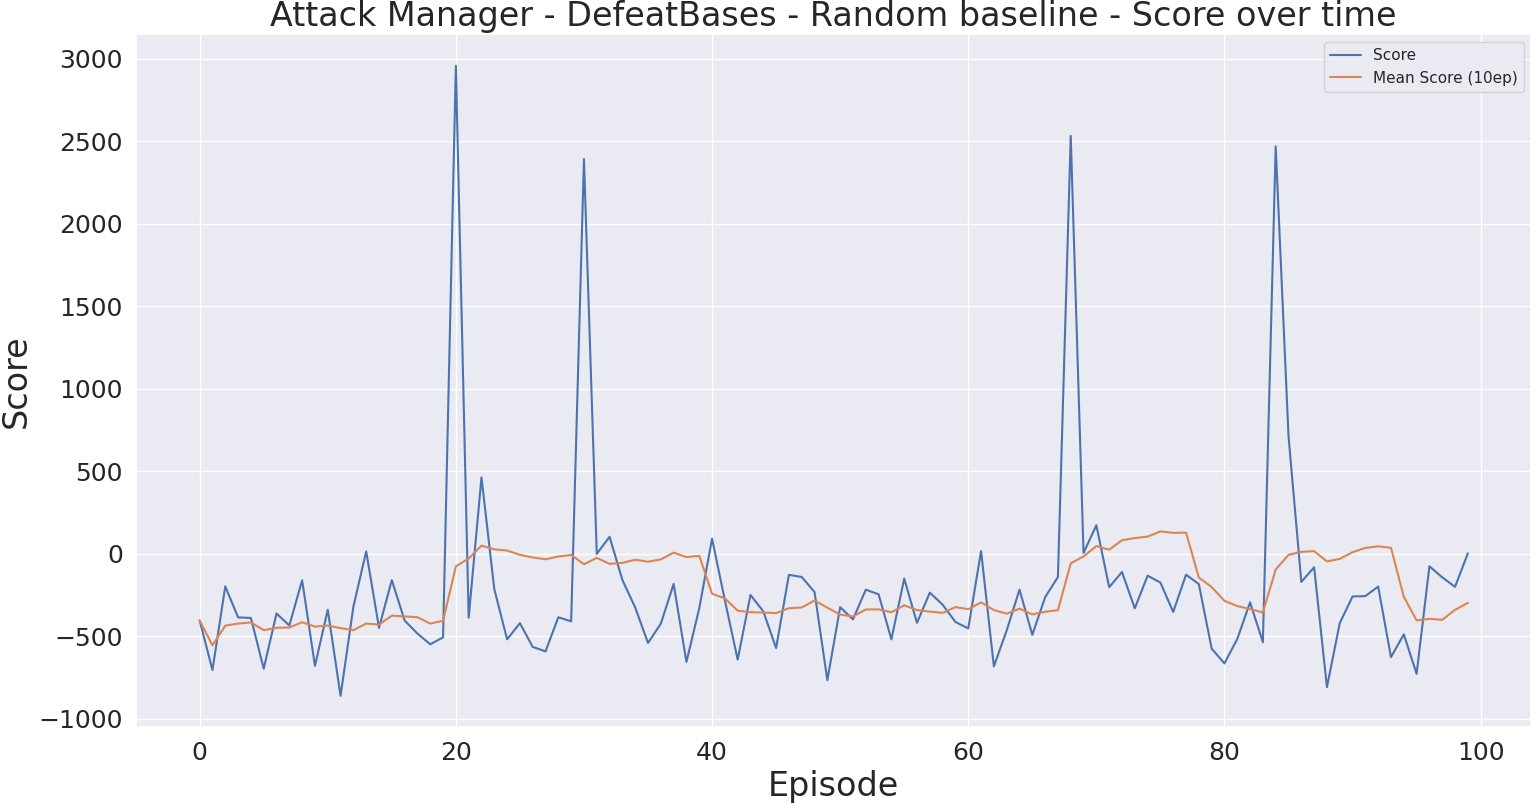
\includegraphics[width=1\textwidth]{figs/multi_random_army_attack_manager/exploit/score.png}
        \caption{Random baseline score}
    \end{subfigure}
    \caption{Scores for \texttt{DefeatBases} mini-game}
    \label{fig:DefeatBases_scores}
\end{figure}

\subsection{Recruit manager}

For this sub-agent we have created a mini-game called \texttt{BuildMarinesFixed} (figure \ref{fig:BuildMarinesFixed}) based on the existing \texttt{BuildMarines} PySC2 mini-game, with a few tweaks to the score handling to adjust it to our training pipeline but keeping the parameters and gameplay of the original unchanged.

The objective of this mini-game is to recruit as many Marines as possible in a limited time frame. The agent starts with one Command Center and 16 SCVs next to a mineral patch, and the map ends after 10 minutes. The agent has to build Supply Depots, Barracks and Marines in the most optimal way possible to maximize the reward.

The first reward signal we decided for this agent was simply a flat reward every time a Marine completed training. This reward has the peculiarity that it is always delayed in time. Since a Marine takes 25 seconds to train, the reward for taking the \texttt{RECRUIT\_MARINE} action will always be received 13 steps later. This shouldn't be a big problem since Q-Learning is capable of handling delayed rewards; and, indeed, the agent was able to learn an effective strategy. However, for reasons explained later in section \ref{sec:hierarchical_agent}, we decided to make the reward signals as instantaneous as possible.

The score for the recruit manager sub-agent is the amount of minerals spent on training marines, and the reward for each step is the change in score. Because the minerals are spent as soon as a Marine begins training and not when it ends, the reward is received immediately. There is no flat penalty every step because the mini-game has a fixed duration so it is not possible to make it end faster

$$
r(t) = \Delta(\texttt{marines\_spending}_{t})
$$

We also experimented penalizing the agent for spending minerals on anything other than Marines, even Supply Depots and Barracks which are necessary to begin training Marines. Our hope was that that would lead to more optimal and less wasteful strategies. While that may still be true, that reward signal caused even more instability during training and exacerbate the convergence difficulties mentioned previously. For that reason, and time limitations, we simplified the reward to the one described above.

While training this sub-agent we noticed that the exploration process was constantly falling into the same patterns. Since Supply Depots are cheaper to build that Barracks and impossible actions are masked, it means that while the agent has enough minerals to build a Supply Depot but not enough to build a Barracks, the only actions it can take are either \texttt{NO\_OP}, or \texttt{BUILD\_SUPPLY\_DEPOT}. The random actions during exploration almost guarantee that the agent would build the Supply Depot before amassing enough minerals to build a Barracks, restarting the process, and only getting to build Barracks once no more Supply Depots could be built. While it wasn't impossible for the agent to randomly build a Barracks before all 24 available Supply Depots, it was infrequent, and building two, three or four Barracks, even more so.

Since the reward signal is never negative, it cannot \say{disuade} the agent from taking certain actions. Because of that, the agent relies heavily on exploration to discover which course of action provides a greater benefit. To favour the exploration process, we have created a second mini-game, \texttt{BuildMarinesRandom} (figure \ref{fig:BuildMarinesRandom}). This map is identical to \texttt{BuildMarinesFixed} except that the scenario can randomly start with one Supply Depot already built, or one Supply Depot and one to four Barracks already built. The more advanced the starting base, the less likely it is. Additionally, the amount of minerals that the agent has at the start of the episode is uniformly distributed from 50 to 500 in increments of 10. This way, we present the agent with different situations to explore.

The agent uses a medium neural network and has been trained for 9000 steps (30 episodes) on \texttt{BuildMarinesRandom} for an initial exploration phase, and then for 9000 steps (30 episodes) more in \texttt{BuildMarinesFixed}, to adapt its strategy to an environment more closely resembling the final versus map. When evaluating the performance of the agent, we use \texttt{BuildMarinesFixed} exclusively, for a standardized environment. Figure \ref{fig:BuildMarinesFixed_scores} shows the scores obtained by the trained agent during exploitation compared to the ones obtained by a random agent.

\begin{figure}[t]
    \centering
    \begin{subfigure}[b]{0.48\textwidth}
        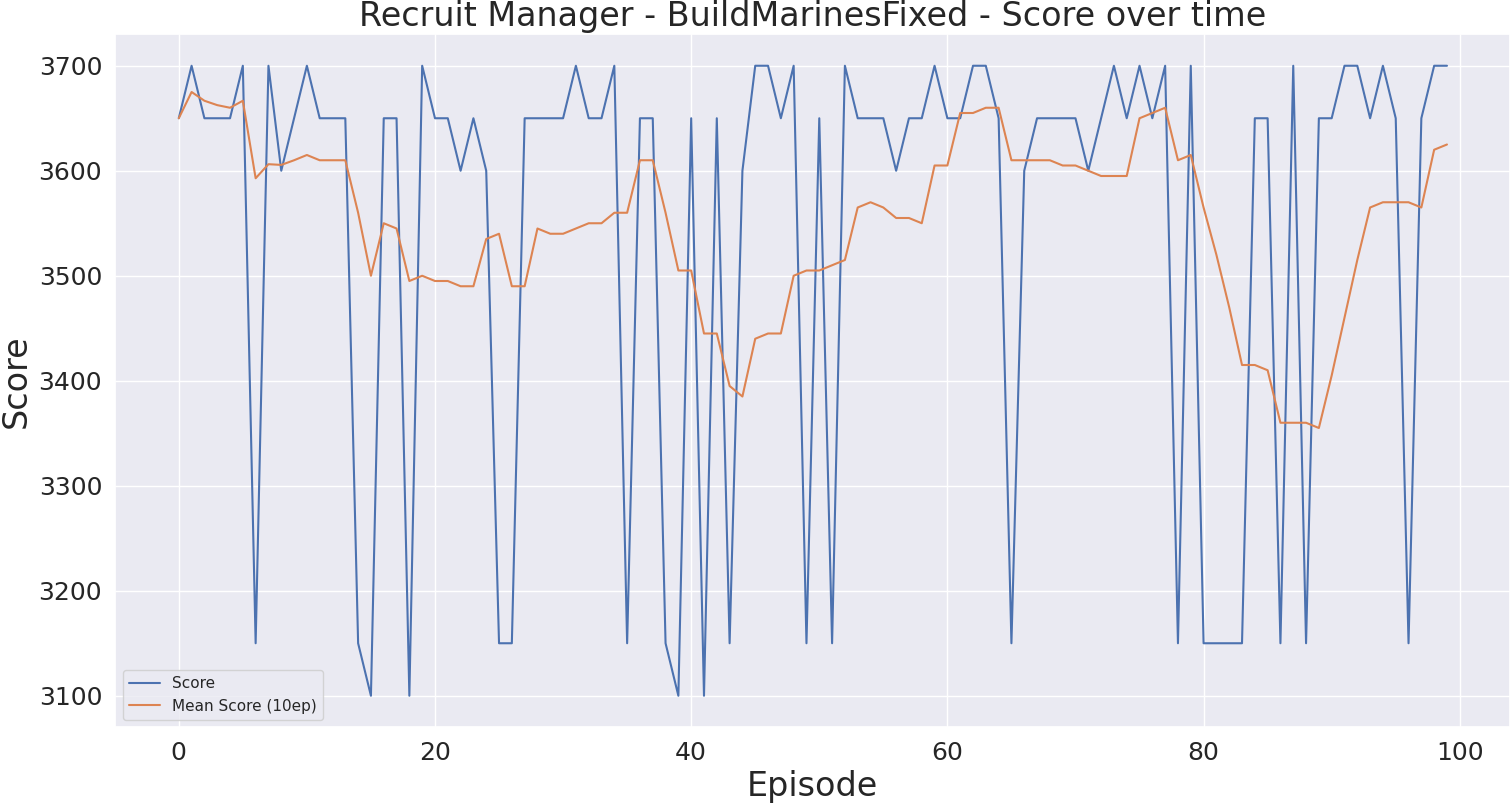
\includegraphics[width=1\textwidth]{figs/multi_dqn_army_recruit_manager/exploit/score.png}
        \caption{Recruit manager sub-agent score}
    \end{subfigure}
    \hfill
    \begin{subfigure}[b]{0.48\textwidth}
        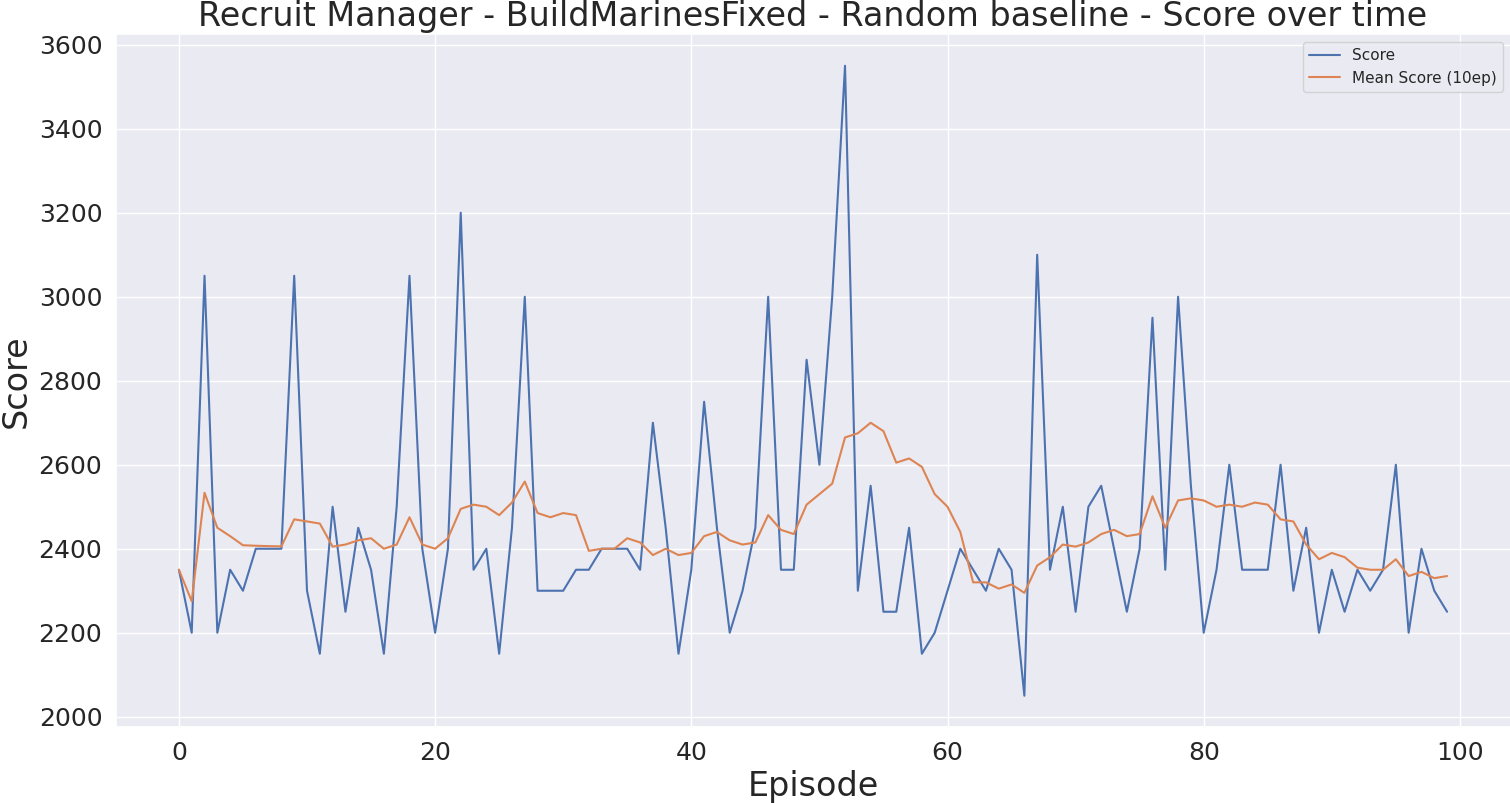
\includegraphics[width=1\textwidth]{figs/multi_random_army_recruit_manager/exploit/score.png}
        \caption{Random baseline score}
    \end{subfigure}
    \caption{Scores for \texttt{BuildMarinesFixed} mini-game}
    \label{fig:BuildMarinesFixed_scores}
\end{figure}

\subsection{Base manager}

One of the mini-games in the PySC2 suite centers around harvesting resources (both minerals and vespene gas) and it is close to what we need for this sub-agent. That map, however, only supports up two bases (two Command Centers), and in the final versus map, the agent can have up to three. Because of that, we have create a new mini-game, \texttt{Saturate\_Harvesters} (figure \ref{fig:SaturateHarvesters}), expanding the existing one and removing the vespene geysers since our agent doesn't make use of them.

The objective of this mini-game is to harvest as many minerals as possible in a limited time frame. The agent starts with one Command Center and eight SCVs next to a mineral patch. The map includes two additional mineral patches to allow for up to two more bases to be built. The map has a fixed duration of 12 minutes.

We experimented with several different reward signals for this map such as the amount of minerals collected since last step, the net change in minerals since las step (which would penalize for spending minerals) and the change in mineral gathering rate (measured in minerals per second). However, all of these are long-term rewards: the benefit of training a new worker and assigning it to harvest minerals is gaining 5 additional minerals every so often for the remainder of the episode. As was the case with the recruit manager, Q-Learning can learn what states lead to better long-term rewards. But as mentioned previously, we favoured the use of immediate reward signals.

We have settled on calculating the score based on the efficiency of the harvesting workers. A Command Center can have any number of workers harvesting resources towards it. However, the optimum number of harvesters depends on the number of nearby mineral deposits. There has been extensive work studying the resource economy of StarCraft II\footnote{\url{https://liquipedia.net/starcraft2/Mining_Minerals}}, but to summarize, for every mineral deposit, the first two workers mining on it will operate at full efficiency, the third worker will operate at roughly half efficiency, and any workers past the third are completely redundant. Since both in the mini-game and in the final versus map each mineral path contains eight mineral deposits, the maximum number of valuable harvesters for each Command Center is 24, with the first 16 being the most valuable. Using that, we calculate the harvesting efficiency score by adding the amount of harvesters up to 16 plus half the amount of harvesters between 16 and 24 on each Command Center. The reward, then, is the change in score from the previous step minus a flat penalty. This way, the reward increases or decreases immediately when an worker is ordered to harvest or when a harvesting worker is ordered to do something else like build a structure. The penalty is removed if the maximum efficiency has been achieved since the agent can no longer improve the efficiency.

$$
r(t) = \Delta(\texttt{harvester\_efficiency}_{t}) - \texttt{step\_cost}
$$

The agent uses a medium neural network and has been trained for 18000 steps (50 episodes). Figure \ref{fig:SaturateHarvesters_scores} shows the scores obtained by the trained agent during exploitation compared to the ones obtained by a random agent.

\begin{figure}[t]
    \centering
    \begin{subfigure}[b]{0.48\textwidth}
        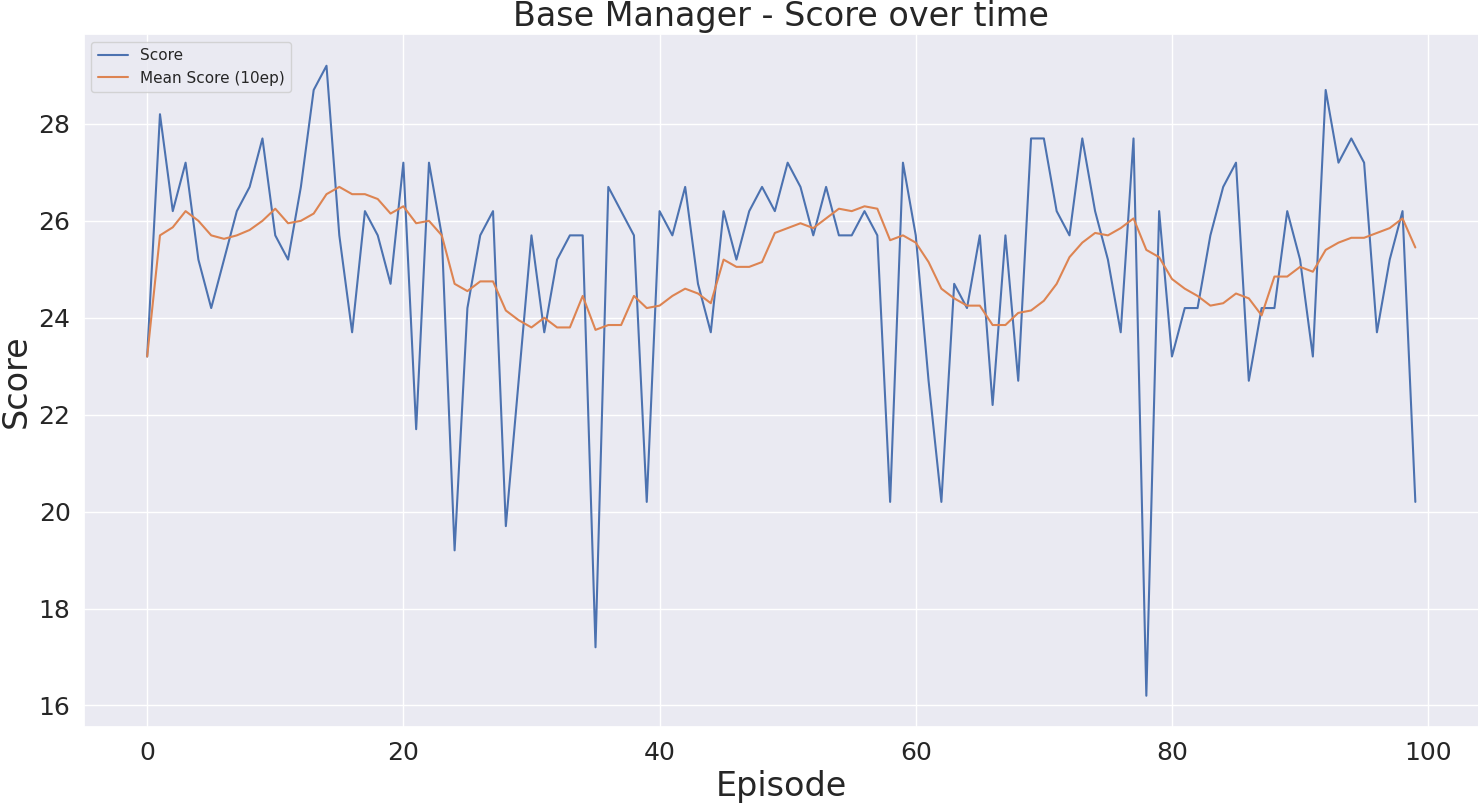
\includegraphics[width=1\textwidth]{figs/multi_dqn_base_manager/exploit/score.png}
        \caption{Base manager sub-agent score}
    \end{subfigure}
    \hfill
    \begin{subfigure}[b]{0.48\textwidth}
        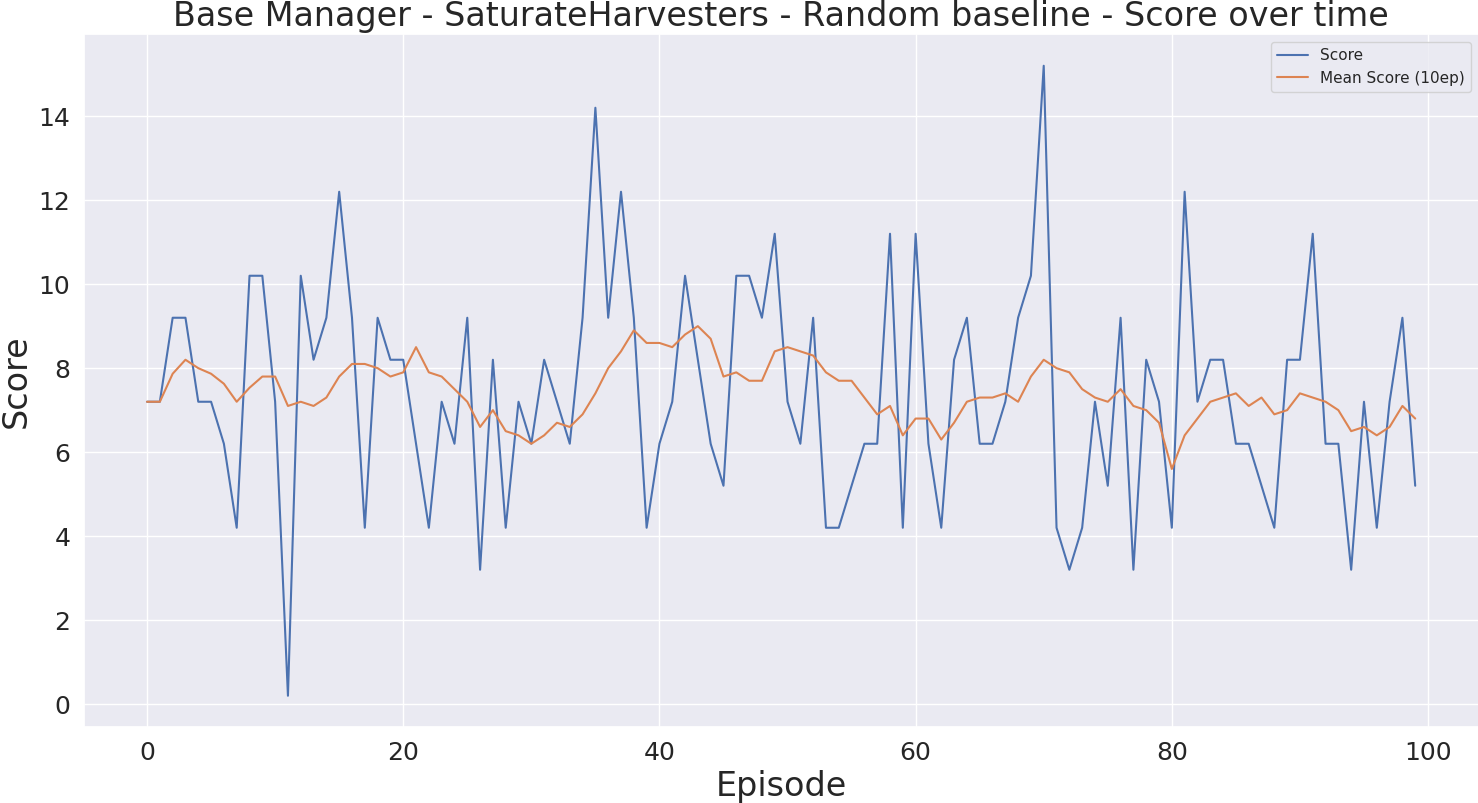
\includegraphics[width=1\textwidth]{figs/multi_random_base_manager/exploit/score.png}
        \caption{Random baseline score}
    \end{subfigure}
    \caption{Scores for \texttt{SaturateHarvesters} mini-game}
    \label{fig:SaturateHarvesters_scores}
\end{figure}

\subsection{Hierarchical agent}
\label{sec:hierarchical_agent}

To train the hierarchical agent we have used the existing PySC2 melee map \texttt{Simple\_64}. It a relatively small \say{Z}-shaped 1v1 versus map. Both players start on opposite corners of the map with a Command Center and 12 SCVs. The remaining two corners hold mineral patches to allow for additional bases. The goal of the map is simply to win the match by destroying all of the opponent's structures. The game can also end in a draw if enough time passes with none of the players being able to gather more resources, produce more units or destroy enemy units. When playing this map, both during training and evaluation, the opponent is controlled by a random agent.

As explained in \ref{sec:reward_signal} using a reward signal based on wins and losses can be problematic due to it being too sparse. We experimented with different ways to calculate the reward until we settled on the following: we calculate a value for both players based on the total mineral value of their units and structured factored by their health percentage (with a minimum factor of $0.5$ since even a badly damaged unit or structure is equally effective at its job). This value is capped at $4000$. The score for the agent, then is the difference between its value and the opponent's, and the reward is the change in score from the previous step with an additional step penalty.

$$
r(t) = \Delta(\max(\texttt{agent\_score}_{t}, 4000) - \max(\texttt{enemy\_score}_{t}, 4000)) - \texttt{step\_cost}
$$

The agent also receives an additional large reward or penalty on the last step of each episode according to the result of the game: $5000$ in case of a victory, $-5000$ in case of defeat and $0$ in case of a draw.

The reason for the maximum score is to disincentivize stalling when a the game is almost over. Without it, the agent could easily get in a position where the enemy is no longer a threat and then keep growing its army at a rate where the reward is greater than the step cost, not only wasting time, but also risking a draw after enough time. This way, past a certain point, the only way to continue getting rewards is to cause damage to the opponent.

The training of the hierarchical agent is divided in two steps: fine-tuning of the sub-agents and training of the main agent.

\subsubsection*{Fine-tuning sub-agents}

In this phase, the main agent and the sub-agents run in combination (with the main agent deciding which sub-agent selects the next actions) for a small number of episodes, with all of them being trained. The goal of this to adjust the sub-agents to the new environment, which is different from the ones each of them have been trained on. Each of the sub-agents receives the same reward signal the did during training.

One problem with this process is that since each sub-agent is only acting about a third of the time, it doesn't experience the states when it isn't acting. This can cause blind spots in an agent's experience that break the chain of states that allow Q-Learning to work. Similarly, the use of delayed and long-term rewards can cause the reward to be received when the sub-agent responsible isn't active, missing it entirely.

To mitigate these issues, we have taken two measures. First, we have avoided as much as possible the use of delayed rewards while training the sub-agents, especially in the case of the recruit manager and the base manager. Second, since all the reward signals are based on comparing a score on the current step with the score of the previous step, for the case of sub-agents, we compare the current score with the score of the last step in which the agent took an action. This means that even if the agent isn't selected to act for several steps, the next time it is selected it will see the change in score from its last action.

The sub-agents have been fine-tuned for 7442 steps combined (20 episodes). At the same time, the main agent uses a medium neural network and has been trained for 1496 steps (20 episodes).

\subsubsection*{Training main agent}

After the fine-tuning process, the sub-agent are frozen and the main agent continues training. The main agent has been trained this way for 3945 additional steps (40 episodes). Figure \ref{fig:hierarchical_Simple64_scores} shows the scores obtained by the trained agent during exploitation compared to the ones obtained by a random agent.

\begin{figure}[t]
    \centering
    \begin{subfigure}[b]{0.48\textwidth}
        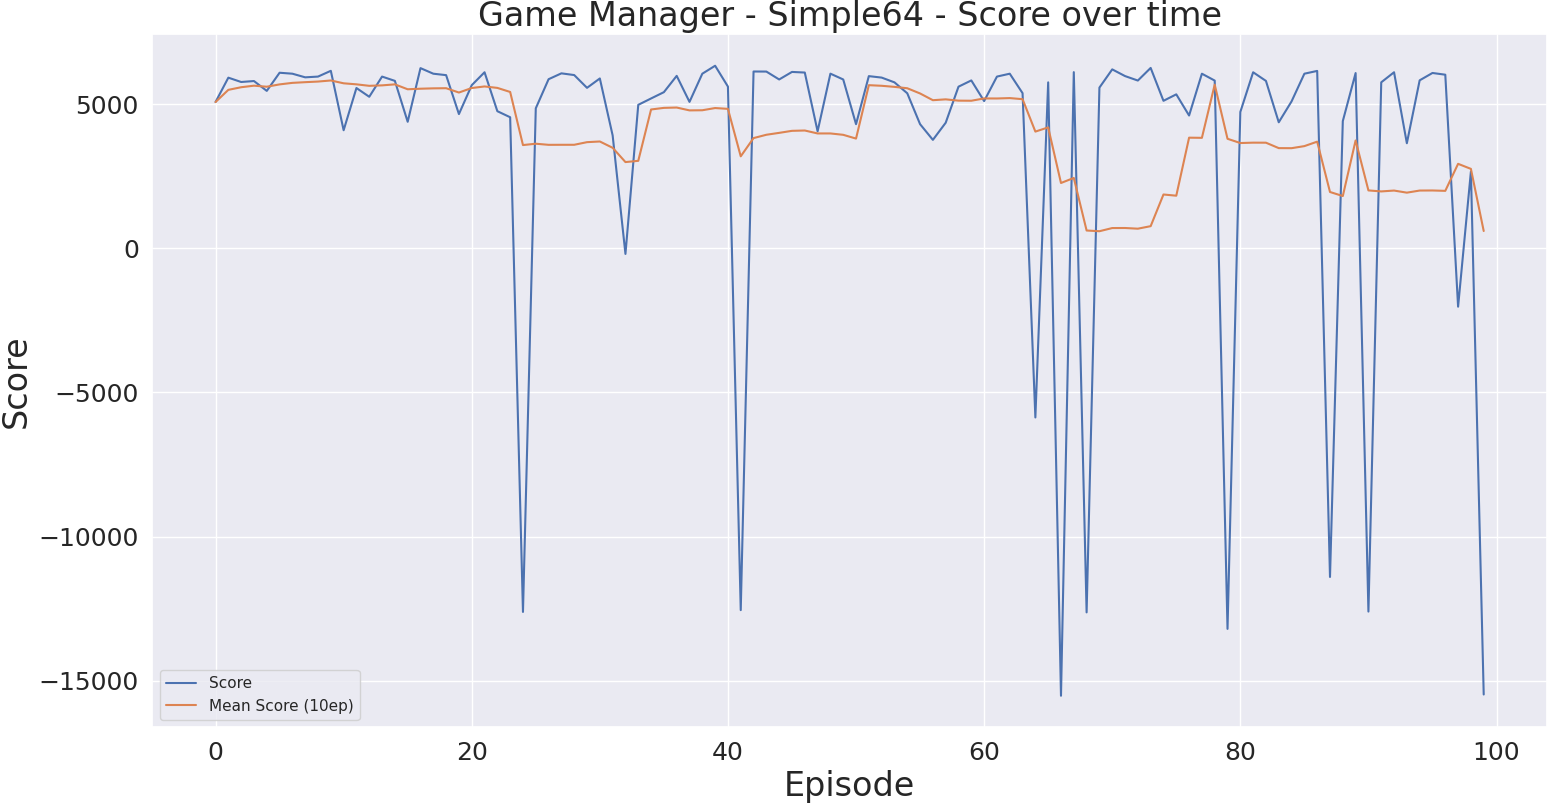
\includegraphics[width=1\textwidth]{figs/multi_dqn_game_manager/exploit/score.png}
        \caption{Hierarchical agent score}
    \end{subfigure}
    \hfill
    \begin{subfigure}[b]{0.48\textwidth}
        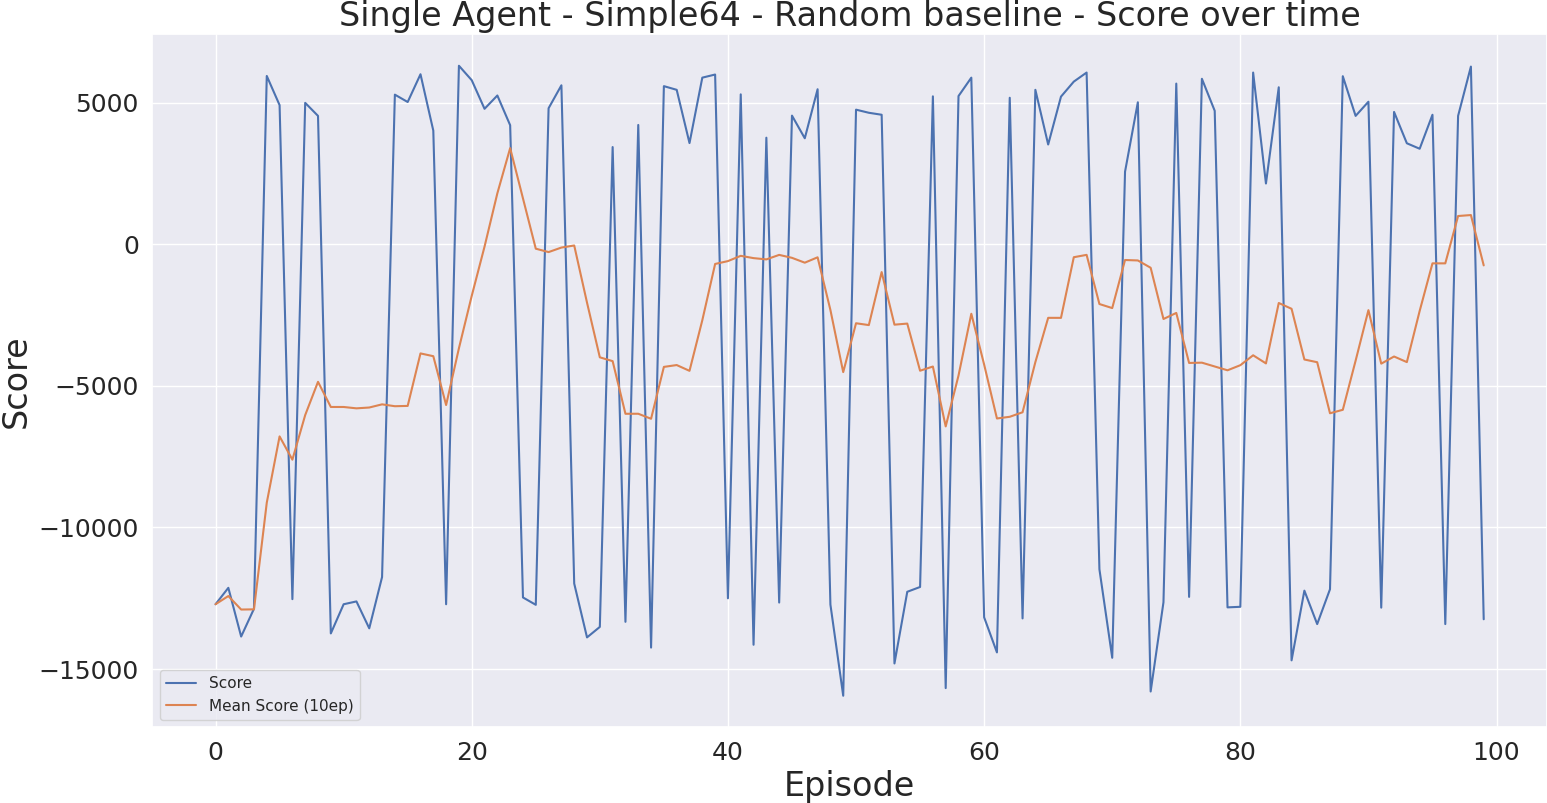
\includegraphics[width=1\textwidth]{figs/single_random/exploit/score.png}
        \caption{Random baseline score}
    \end{subfigure}
    \caption{Scores for hierarchical agent in \texttt{Simple64} map}
    \label{fig:hierarchical_Simple64_scores}
\end{figure}

\subsection{Single agent}

Finally, for the single RL agent that is to be used as the control for the performance and efficiency of the hierarchical agent we have trained two agents. The first agent is meant to be as good as possible while being limited to the same training cost as the hierarchical agent, and, conversely, the second is meant to match the performance of the hierarchical agent regardless of the training efficiency. Both agents haven been trained with the same environment and reward signal as the hierarchical agent.

The first agent uses a medium network (the same size as the networks of all hierarchical sub-agents) and has been trained for 52572 steps (130 episodes). For the second agent, we needed to upgrade to a large network to come close to the same performance. It has been trained for 79768 steps (200 episodes). Figure \ref{fig:hierarchical_Simple64_scores} shows the scores obtained by both agents during exploitation compared to the ones obtained by a random agent.

\begin{figure}[t]
    \centering
    \begin{subfigure}[b]{0.48\textwidth}
        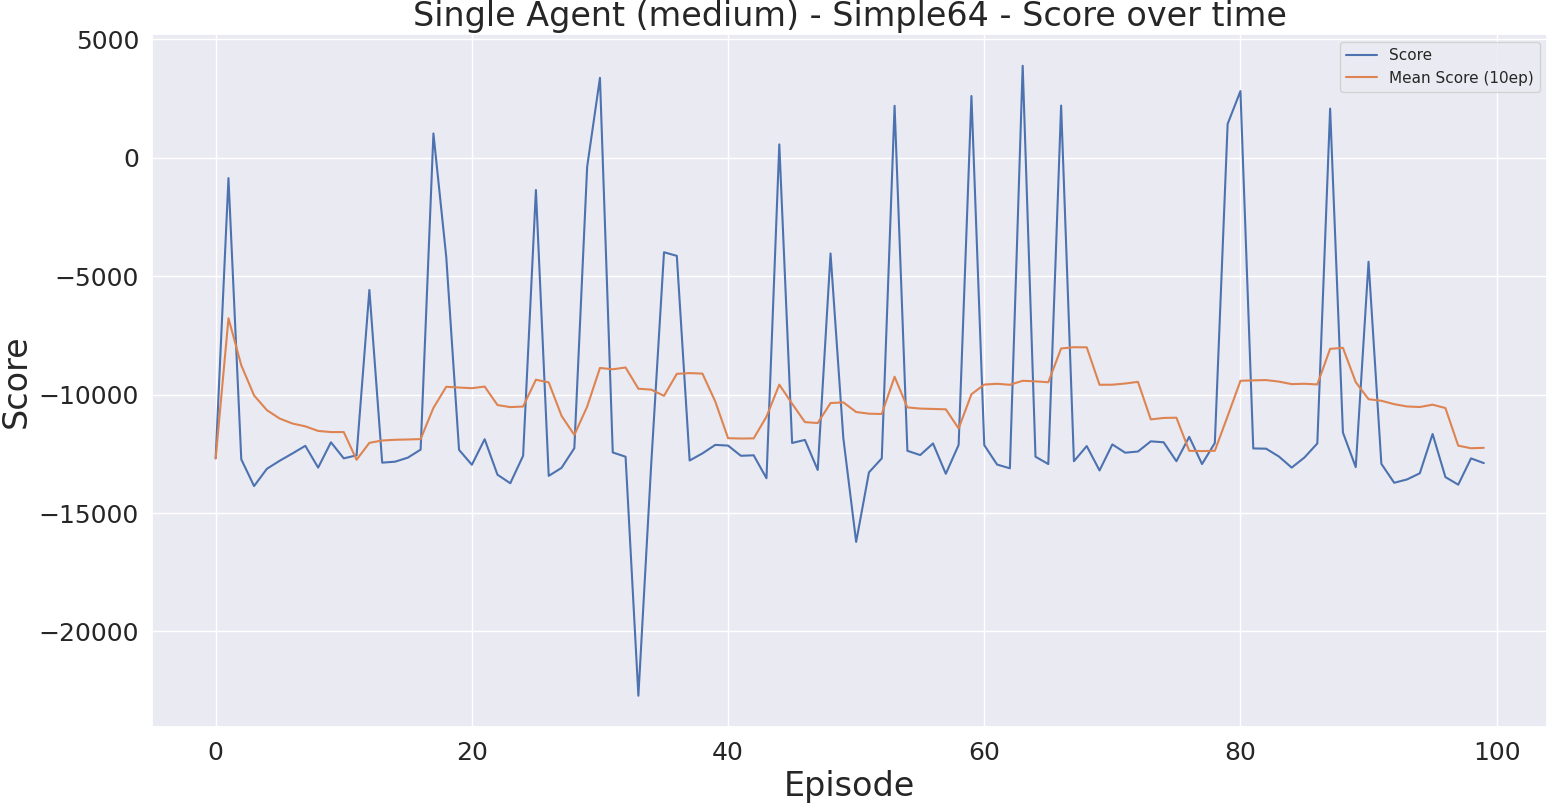
\includegraphics[width=1\textwidth]{figs/single_dqn_m_130/exploit/score.png}
        \caption{Single agent (medium) score}
    \end{subfigure}
    \hfill
    \begin{subfigure}[b]{0.48\textwidth}
        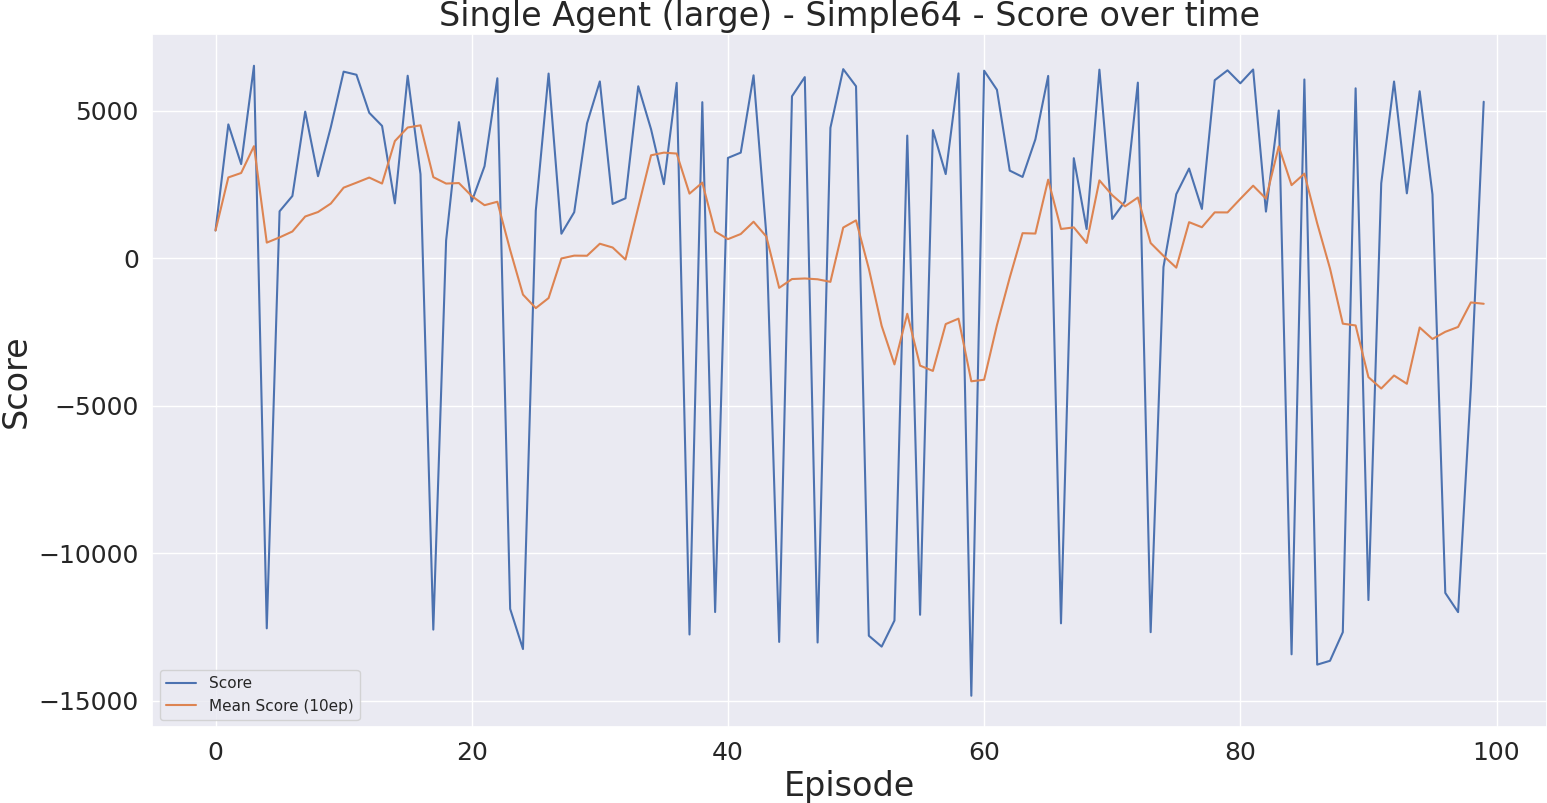
\includegraphics[width=1\textwidth]{figs/single_dqn_l_200/exploit/score.png}
        \caption{Single agent (large) score}
    \end{subfigure}
    \hfill
    \begin{subfigure}[b]{0.48\textwidth}
        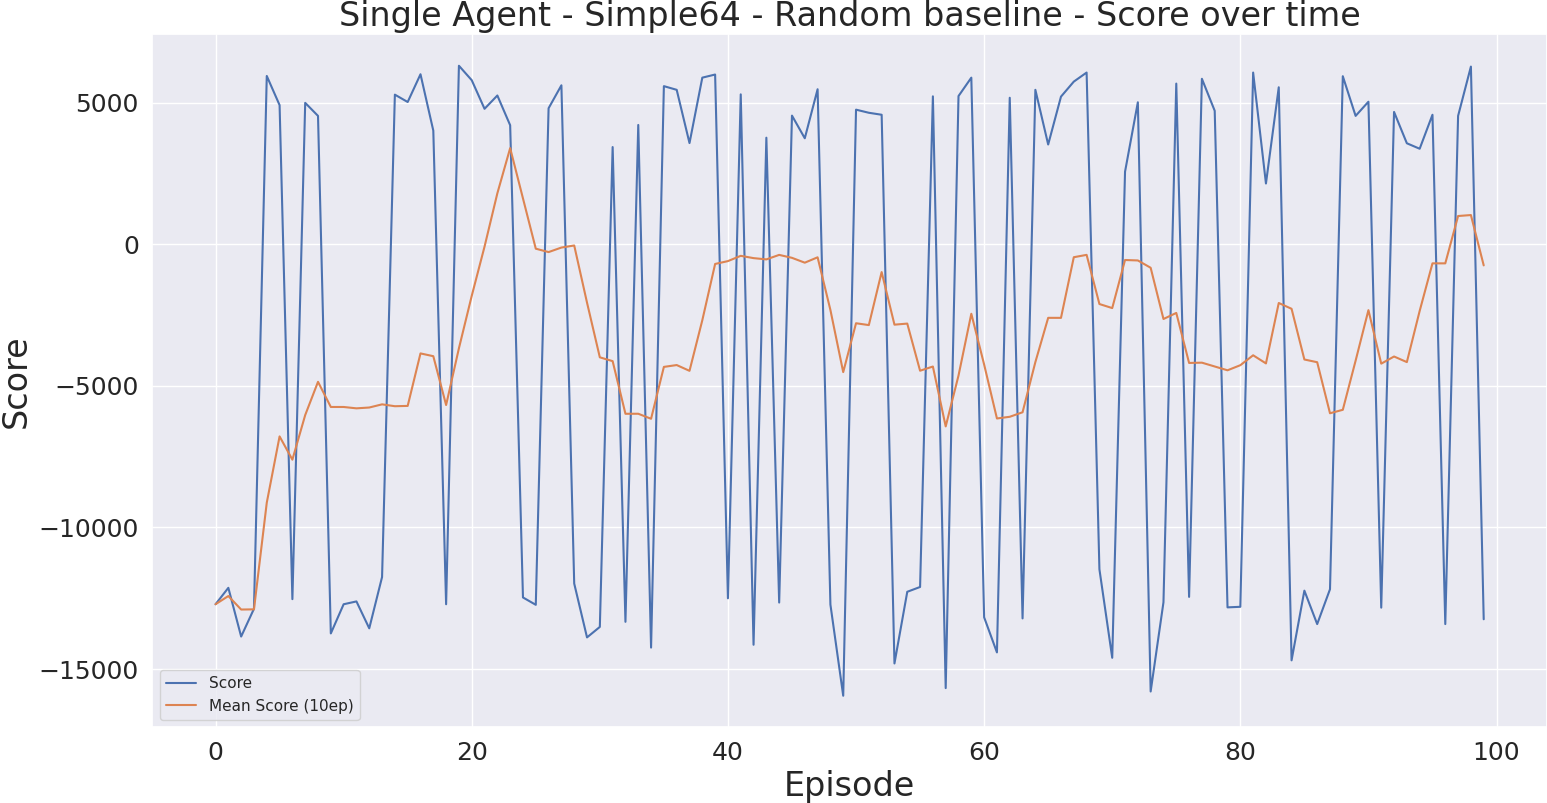
\includegraphics[width=1\textwidth]{figs/single_random/exploit/score.png}
        \caption{Random baseline score}
    \end{subfigure}
    \caption{Scores for single agent in \texttt{Simple64} map}
    \label{fig:single_Simple64_scores}
\end{figure}

\section{Results}

\begin{table}[t]
    \centering
    \begin{tabular}{ l|c l l l }
        & Performance & Energy (kW/h) & CO\textsubscript{2} emissions (kg) & FPOs \\
        \hline \hline
        Single agent M & \cellcolor{Maroon!25}$13$/$8$/$79$ ($13.00\%$) & \cellcolor{Dandelion!25}$0.09202$ & \cellcolor{Dandelion!25}$0.015547$ & \cellcolor{OliveGreen!25}$1.93\mathrm{e}12$ \\
        Single agent L & \cellcolor{Dandelion!25}$78$/$0$/$22$ ($78.00\%$) & \cellcolor{Maroon!25}$0.12199$ & \cellcolor{Maroon!25}$0.020814$ & \cellcolor{Maroon!25}$6.32\mathrm{e}12$ \\
        Hierarchical agent & \cellcolor{OliveGreen!25}$91$/$3$/$6$ ($91.00\%$) & \cellcolor{OliveGreen!25}$0.0889$ & \cellcolor{OliveGreen!25}$0.0150$ & \cellcolor{Dandelion!25}$2.02\mathrm{e}12$ \\
        \hline
        \quad Base manager & --- & $0.0207$ & $0.00349$ & $6.61\mathrm{e}11$ \\
        \quad Recruit manager & --- & $0.0225$ & $0.00380$ & $6.61\mathrm{e}11$ \\
        \quad Attack manager & --- & $0.00575$ & $0.000972$ & $2.26\mathrm{e}11$ \\
        \quad Game manager & --- & $0.0401$ & $0.00677$ & $4.71\mathrm{e}11$ \\
    \end{tabular}
    \caption{Results summary}
    \label{tab:results}
\end{table}

\begin{figure}[t]
    \centering
    \begin{subfigure}[b]{0.48\textwidth}
        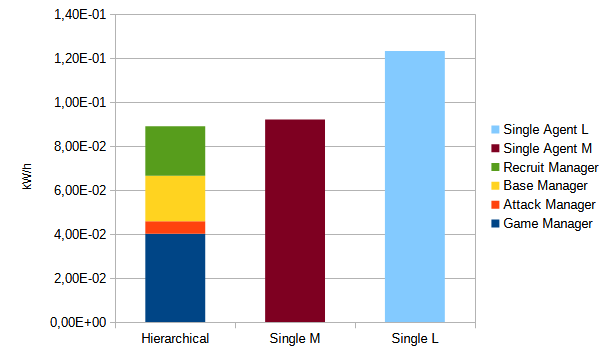
\includegraphics[width=1\textwidth]{figs/training_energy.png}
        \caption{Energy consumed}
    \end{subfigure}
    \hfill
    \begin{subfigure}[b]{0.48\textwidth}
        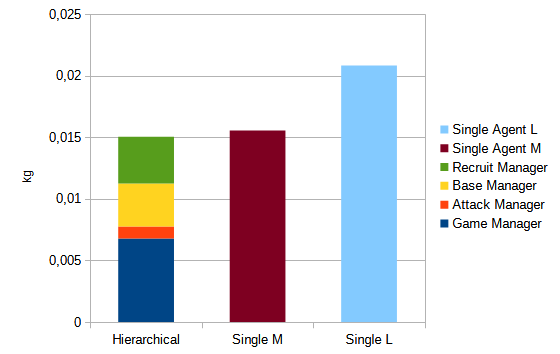
\includegraphics[width=1\textwidth]{figs/training_emissions.png}
        \caption{Carbon emissions}
    \end{subfigure}
    \hfill
    \begin{subfigure}[b]{0.48\textwidth}
        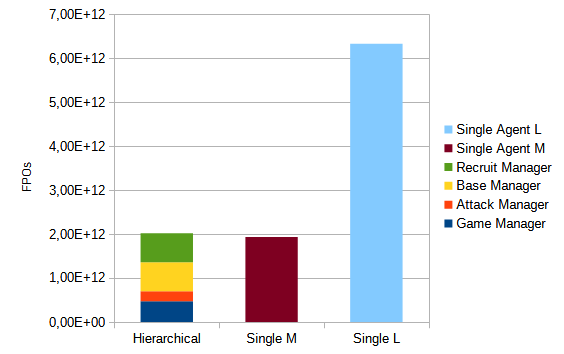
\includegraphics[width=1\textwidth]{figs/training_fpos.png}
        \caption{FPOs performed}
    \end{subfigure}
    \caption{Training efficiency summary}
    \label{fig:results}
\end{figure}

Table \ref{tab:results} lists a summary of the results we have obtained, which are also visualized in figure \ref{fig:results}. After training was complete, we have measured the performance the hierarchical agent and the two single agents by making them play 100 games in \texttt{Simple\_64} against a random agent. The hierarchical agent has achieved a 91\% win rate. The large single agent has had a worse, but still positive performance with a 78\% win rate, while the medium single agent has performed considerably worse than random, winning only 13\% of the games.

To measure the efficiency of the different agents during training, we have used the codecarbon\footnote{\url{https://codecarbon.io/}} Python library, which periodically measures the energy consumed by the hardware (CPU, GPU, etc.) and estimates the carbon emissions that would be generated by producing that amount of energy. However, due to hardware and operating system incompatibilities, codecarbon was not able to access the hardware on our setup, so all the measurements are a brute estimation based on a theoretical constant consumption. We include these values in the summary table for the sake of completeness, but they are not particularly accurate.

An alternative way to estimate the training cost of our models is to obtain the number of floating-point operations (FPOs) that are performed \cite{Schwartz:2019}. FPOs serve as an estimate of the work performed by a computational process, and using them as a measure has the advantage that it is independent of the hardware. While we can't obtain the exact number of FPOs performed during training, we can approximate them based on the size of the neural networks and the number of inferences and backpropagations executed.

For a completely connected neural network like the ones we use, the number of weights of each layer is equal to the product of the number of neurons in the layer and the number of neurons in the next layer. Our networks have 68 inputs and 15 outputs, except for the case of the hierarchical main agent, which has only 3 outputs, and the number of hidden layers and nodes depends on the sizes described in section \ref{sec:agent_structure}. The resulting amounts of weights for each network size are listed in table \ref{tab:weights}.

\begin{table}[h]
    \centering
    \begin{tabular}{ l|r r }
        Network size & Weights & Weights (game manager) \\
        \hline
        Medium & $35808$ & $35424$ \\
        Large & $77280$ & $76896$ \\
        Extra large & $225760$ & $225376$ \\
    \end{tabular}
    \caption{Number of weights of the neural networks}
    \label{tab:weights}
\end{table}

Following the DQN algorithm (algorithm \ref{alg:dqn2}), we can calculate the number of operations executed by each neural network of an agent. During training, the main network performs one inference on every step\footnote{Due to the $\epsilon$-greedy method, the agent doesn't actually calculate an action every step. However, even when taking that into account, the difference in the final calculation is four orders of magnitude smaller than the total result.} to select an action for the agent to take. Also every step, both the main and target network perform one inference for every experience in the update batch to estimate the q-value of the sample. Lastly, after the loss and gradients are calculated, the main network is updated through backpropagation. This results in the following formula to estimate the number of FPOs performed by the networks:

\begin{equation}
    \mathrm{FPO} \approx W \cdot (S + 2SJ + S) = 2WS(J+1)
\end{equation}

Where $W$ is the number of weights in the network, $S$ is the number of steps taken during training and $J$ is the learning batch size, which in our case is 512 for all agents.

After calculating the FPOs for each agent we see that training the single large agent involves 3 times more floating-point operations than the entire group of hierarchical agents.